\section{Approach}
\label{sec:kv}
\begin{figure}[t]
	\centering
	\scalebox{0.55}{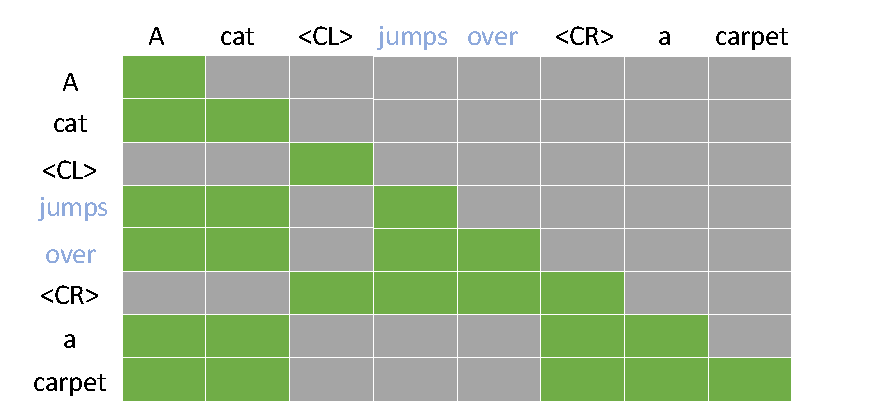
\includegraphics{./figures/attention_2.pdf}}
  \caption{Modified attention mask for context compression. Green and grey boxes indicate positions that are allowed and disallowed to be attended to~(attention direction from row $\rightarrow$ column).}
	\label{fig:kv}
\end{figure}

In this section, we present a plug-and-play approach to compress the full-length contextual representations into shorter ones while preserving information necessary to accomplish the end task.

\subsection{Context Compression with Sentinel Tokens}
To alleviate the computational and memory intensity of key-value memory when processing increasingly long context, we introduce two sentinel tokens \textit{<CL>} and \textit{<CR>} into the vocabulary of LLM, that are placed around a contiguous span of tokens of which the corresponding key-value memory will be compressed. 

\begin{table*}[th]
\small
\centering
\begin{tabular}{c|c|cccccccccc}
\toprule
  \multirow{2}{*}{Model}        & \multirow{2}{*}{Method} & \multicolumn{10}{c}{Compression Ratio~($r$)}                                                                                                                                                                         \\
                              &                 & \multicolumn{1}{c}{0.0}  & \multicolumn{1}{c}{0.1}      & \multicolumn{1}{c}{0.2} & \multicolumn{1}{c}{0.3} & \multicolumn{1}{c}{0.4} & \multicolumn{1}{c}{0.5} & \multicolumn{1}{c}{0.6} & \multicolumn{1}{c}{0.7} & \multicolumn{1}{c}{0.8} & \multicolumn{1}{c}{0.9} \\
\midrule
  \multirow{3}{*}{OPT-1.3B}     & Scattered Attention  & \multicolumn{1}{c}{15.0}  & \multicolumn{1}{c}{18.2} & \multicolumn{1}{c}{22.6}    & \multicolumn{1}{c}{28.2}    & \multicolumn{1}{c}{35.8}    & \multicolumn{1}{c}{47.2}    & \multicolumn{1}{c}{59.6}    & \multicolumn{1}{c}{81.0}    & \multicolumn{1}{c}{106.4}    & \multicolumn{1}{c}{151.6}    \\

                              & Local Attention    &15.0   &15.1  & \textbf{15.2}                    & 15.7                    & 16.3                    & \textbf{17.2}                    & 18.2                    & 19.9                    & 23.0                    & 29.8                    \\
                              & KV Compression      &15.0  &\textbf{15.0}  & \textbf{15.2}                    & \textbf{15.6}                    & \textbf{15.9}                    & 17.3                    & \textbf{17.8}                    & \textbf{18.0}                    & \textbf{18.1}                    & \textbf{18.3}                    \\
 \midrule
  \multirow{3}{*}{OPT-2.7B}     & Scattered Attention    &13.1 &16.2  & 19.8                    & 25.5                    & 32.4                    & 41.7                    & 56.3                    & 75.7                    & 101.4                   & 142.3                   \\
                              & Local Attention     &13.1   &\textbf{13.1} & \textbf{13.4}                    & 13.9                    & 14.4                    & 15.3                    & 16.1                    & 17.5                    & 20.1                    & 26.6                    \\
                              & KV Compression       &13.1 &13.2  & 13.5                    & \textbf{13.7}                    & \textbf{14.0}                    & \textbf{15.3}                    & \textbf{15.8}                    & \textbf{16.0}                    & \textbf{16.1}                    & \textbf{16.3}                    \\
 \midrule
  \multirow{3}{*}{RedPajama-3B} & Scattered Attention  &11.2 &13.1  & 16.5                    & 20.7                    & 26.6                    & 34.9                    & 47.2                    & 65.7                    & 91.6                    & 135.9                   \\
                              & Local Attention      &11.2  &\textbf{11.3} & \textbf{11.5}                    & \textbf{11.8}                    & 12.2                    & 12.9                    & 13.6                    & 14.8                    & 17.2                    & 22.9                    \\
                              & KV Compression      &11.2  &11.4  & \textbf{11.5}                    & \textbf{11.8}                   & \textbf{11.9}                    & \textbf{12.3}                    & \textbf{13.5}                    & \textbf{13.7}                    & \textbf{13.8}                    & \textbf{14.0}               \\    
\bottomrule
\end{tabular}
\caption{Perplexity~(the lower the better) of three LLMs on WikiText-2 language modeling benchmark.
}
% \KZ{In terms of perplexity, kv is not too much better than
% local attention, it seems. So we should try to demo kv's advantage in some
% other perspectives?}}
\label{table:main}
\end{table*}
In order to consolidate information of tokens surrounded by \textit{<CL>} and \textit{<CR>}, we design a modified causal attention mask to facilitate such behaviour. An illustrative example is shown in \figref{fig:kv}. 
Specifically, \textit{<CL>} serves a start-of-compression symbol and can only attend to itself. Normal tokens~(tokens except for \textit{<CL>} and \textit{<CR>}) have access to all previous \textit{<CR>} and normal tokens. This ensures that the contextual representations are built upon both compressed~(lossy) and complete~(lossless) past information. \textit{<CR>} then act as a form of information selection and retrieval from contextual representations of surrounded tokens. This modified masking scheme, combined with task-specific fine-tuning of LLM, encourages distilling task-relevant information of potentially long token sequences into a compact representation, thereby reducing the size of key-value memory required for subsequent processing.

\paragraph{Input Transformation} Given an input $\bm{x}$ with $L$ tokens, 
we define compression ratio $r$ as the percentage of the tokens
to be enclosed by one or more pairs of \textit{<CL>} and \textit{<CR>},
and max compression length $l$ as 
 the largest number of tokens to be compressed by a single pair of 
\textit{<CL>} and \textit{<CR>} tokens. 
We repeatedly sample span of tokens with length conforming to a uniform distribution $\bm{U}(2,l)$ as compression target, until ratio $r$ is reached. 
But these spans must not overlap. 
We tie the position encoding of \textit{<CL>} and \textit{<CR>} to their previous token, such that they don't occupy valuable positions for 
LLMs using absolute position embedding.

\paragraph{Training} We opt for a light-weight procedure for adapting LLMs to downstream tasks through fine-tuning. 
Specifically, all parameters of the LLM are frozen except for the embeddings 
of \textit{<CL>} and \textit{<CR>} and LoRA~\cite{lora} modules applied to 
all attention layers. This not only eases the training process of models 
with billions of parameters but also ensures the inherent language modeling 
ability and parametric knowledge in feedforward networks are 
intact~\cite{keyvalue}.
\paragraph{Manipulating Key-Value Memory for Inference-time Compression} 
Given a text piece as prefix, we apply the same input transformation strategy defined above to reach a specified compression ratio. To realize perceivable memory and computation reduction, the key-value cache of tokens enclosed by sentinel tokens is freed from GPU in a progressive manner~(e.g., using a for-loop over blocks of tokens) if the original prefix is too long to fit into GPU. Otherwise we just feed the transformed prefix through the model and free the key-value cache of marked tokens in one go.